%
% Presentación para congreso.
% Proyecto Lovelace.
%

\documentclass{beamer}
\usepackage{formato}
\usepackage{array}
\newcommand{\Titulo}{Un vistazo a la tokenización}
\newcommand{\Fecha}{Puebla, 14 de octubre de 2018}
\usepackage{formato_presentaciones}

\renewcommand{\Autor}{Daniel Ayala Zamorano \\\vspace{-2mm}
  {\tiny \texttt{daz23ayala@gmail.com}} \\
  Laura Natalia Borbolla Palacios \\\vspace{-2mm}
  {\tiny \texttt{ln.borbolla.42@gmail.com}} \\
  Ricardo Quezada Figueroa \\\vspace{-2mm}
  {\tiny \texttt{qf7.ricardo@gmail.com}} \\
  Sandra Díaz Santiago \\\vspace{-2mm}
  {\tiny \texttt{sdiazs@gmail.com}}}

\setbeameroption{show notes}

\usepackage[caption=false,font=footnotesize]{subfig}
\usepackage{tikz}
\usetikzlibrary{
  arrows.meta,
  decorations.pathmorphing,
  backgrounds,
  positioning,
  calc,
  scopes,
  shapes}

\tikzset{
  font=\tiny}

\begin{document}

  {\setbeamertemplate{footline}{}
  \frame{\titlepage}}

  \begin{frame}
    \frametitle{Contenido}
    \setcounter{tocdepth}{1}
    \tableofcontents
  \end{frame}

  % Espacio entre párrafos
  \setlength{\parskip}{0.5em}

  \section{El problema de la protección de datos bancarios}

  \begin{frame}{El problema de la protección de datos bancarios}
    \begin{itemize}
      \item El crecimiento del comercio en línea, aunado a sistemas débilmente
        protegidos propició un incremento en los robos de datos bancarios.
      \item En el 2004 se publicó el PCI DSS\footnotemark \cite{pci_dss}.
      \item Hasta este momento el enfoque era proteger la información en donde
        sea que se encuentre.
      \item A pesar de la publicación del estándar, las filtraciones de datos
        no han cesado.

    \end{itemize}
    \footnotetext{\textit{Payment Card Industry, Data Security Standard}}
  \end{frame}

  \section{La tokenización en otros contextos}

  \begin{frame}{La tokenización en otros contextos}
    Como:
    \begin{itemize}
      \item Moneda de uso particular sin valor legal.
      \item Componente de seguridad en la comunicación por sesiones.
      \item Componente léxico de una gramática.
      \item Una unidad lingüística básica.
      \item Problema social.
    \end{itemize}
  \end{frame}

  \section{¿Qué es la tokenización?}

  \begin{frame}{¿Qué es la tokenización en criptografía?}
    \begin{itemize}
      \item Es la sustitución de datos sensibles por valores representativos
        sin una relación directa.
      \item Existen muchas empresas que proveen el servicio de tokenización,
        pero lo hacen sin detallar la forma en la que se
        realiza~\cite{shif4_uno, braintree_uno, securosis}.
      \item En 2011, el PCI publicó su guía de tokenización~\cite{pci_tokens}.
    \end{itemize}

    \begin{figure}
      \centering
      \begin{tikzpicture}[
        entorno/.style={
          rectangle,
          draw = black,
          thin,
          inner sep = 1mm,
          text width = 15mm,
          align = center,
          minimum height = 1.0cm},
        etiqueta/.style={
          align = center
        }]

        \node[entorno]
          (usuario)
          {Usuario};
        \node[entorno]
          (tienda)
          [right = of usuario]
          {Tienda en línea};
        \node[entorno]
          (sistema_tokenizador)
          [right = of tienda]
          {Sistema tokenizador};
        \only<2>{
          \node[entorno]
            (banco)
            [right = of sistema_tokenizador]
            {Entorno bancario};}

        \draw[-Stealth]
          ($(usuario.north) + (0.1in, 0)$)
          --
          ($(usuario.north) + (0.1in, 0.1in)$)
          --
          node[
            etiqueta,
            above]
            {1.
              \only<1>{Tarjeta: \\ \texttt{1234567891234567}}
              \only<2>{Petición de \\ compra}}
          ($(tienda.north) + (-0.1in, 0.1in)$)
          --
          ($(tienda.north) + (-0.1in, 0)$);

        \draw[-Stealth]
          ($(tienda.north) + (0.1in, 0)$)
          --
          ($(tienda.north) + (0.1in, 0.1in)$)
          --
          node[
            etiqueta,
            above]
            {2.
              \only<1>{Tarjeta: \\ \texttt{1234567891234567}}
              \only<2>{Petición de \\ compra}}
          ($(sistema_tokenizador.north) + (-0.1in, 0.1in)$)
          --
          ($(sistema_tokenizador.north) + (-0.1in, 0)$);

        \only<2>{
          \draw[-Stealth]
            ($(sistema_tokenizador.north) + (0.1in, 0)$)
            --
            ($(sistema_tokenizador.north) + (0.1in, 0.1in)$)
            --
            node[
              etiqueta,
              above]
              {3. Petición de \\ transacción}
            ($(banco.north) + (-0.1in, 0.1in)$)
            --
            ($(banco.north) + (-0.1in, 0)$);

          \draw[-Stealth]
            ($(banco.south) + (-0.1in, 0)$)
            --
            ($(banco.south) + (-0.1in, -0.1in)$)
            --
            node[
              etiqueta,
              below]
              {4. Resultado de \\ operación}
            ($(sistema_tokenizador.south) + (0.1in, -0.1in)$)
            --
            ($(sistema_tokenizador.south) + (0.1in, 0)$);}

        \draw[-Stealth]
          ($(sistema_tokenizador.south) + (-0.1in, 0)$)
          --
          ($(sistema_tokenizador.south) + (-0.1in, -0.1in)$)
          --
          node[
            etiqueta,
            below]
            {\only<1>{3. Token: \\ \texttt{2954634586102951}}
             \only<2>{5. Resultado de \\ operación}}
          ($(tienda.south) + (0.1in, -0.1in)$)
          --
          ($(tienda.south) + (0.1in, 0)$);

        \draw[-Stealth]
          ($(tienda.south) + (-0.1in, 0)$)
          --
          ($(tienda.south) + (-0.1in, -0.1in)$)
          --
          node[
            etiqueta,
            below]
            {\only<1>{4}\only<2>{6}. Resultado de \\ operación}
          ($(usuario.south) + (0.1in, -0.1in)$)
          --
          ($(usuario.south) + (0.1in, 0)$);

      \end{tikzpicture}
      \caption{Arquitectura de sistema tokenizador:
        \only<1>{operación de tokenización}%
        \only<2>{transacción bancaria}.}
    \end{figure}
  \end{frame}

  \section{Clasificación del PCI}

  \begin{frame}{Clasificación de los algoritmos tokenizadores}
    \begin{center}
      \begin{columns}
        \begin{column}{0.5\textwidth}
          Clasificación del PCI \cite{pci_tokens}:
          \vspace{1.0em}
          \begin{itemize}
            \item Reversibles
            \begin{itemize}
              \item Criptográficos
              \item No criptográficos
            \end{itemize}
            \item Irreversibles
            \begin{itemize}
              \item Autenticables
              \item No autenticables
            \end{itemize}
          \end{itemize}
        \end{column}
        \begin{column}{0.5\textwidth}
          Clasificación propuesta:
          \vspace{1.0em}
          \begin{itemize}
            \item Criptográficos
            \begin{itemize}
              \item Reversibles
              \item Irreversibles
            \end{itemize}
            \item No criptográficos
            \begin{itemize}
              \item[]
              \item[]
            \end{itemize}
          \end{itemize}
        \end{column}
      \end{columns}
    \end{center}
  \end{frame}

  \section{Métodos reversibles: FFX y BPS}

  \begin{frame}{Métodos reversibles: FFX y BPS}

    \begin{itemize}
      \item Métodos que utilizan cifrados que preservan el formato.
      \item Cifran la tarjeta y descifran el token.
      \item Se volvieron estándares en 2016 y fueron renombrados por el NIST
        a FF1 y FF3 respectivamente.
      \item Están basados en redes Feistel.
    \end{itemize}

  \end{frame}

  \begin{frame}{Comparativa: FFX y BPS}

    \begin{table}
      \begin{tabular}{|m{0.35\textwidth}|m{0.26\textwidth}|m{0.25\textwidth}|}
        \hline
        \textbf{Características} & \textbf{FFX} & \textbf{BPS}
        \\\hline
        Longitud de cadena & [4,36] caracteres & hasta $56 \cdot 2^{128}$ caracteres
        \\\hline
        Primitiva criptográfica & AES CBC-MAC & AES
        \\\hline
        Tamaño de llave & 128 bits & 128 bits
        \\\hline
        Tamaño de \textit{tweak} & menor a $2^{64}$ bits & 64 bits
        \\\hline
        Número de rondas & 12, 28 o 24 & 8 recomendadas
        \\\hline
      \end{tabular}
      \caption{Comparativa de FFX y BPS.}
    \end{table}

  \end{frame}

  \section{Métodos irreversibles: TKR, AHR y DRBG}

  \begin{frame}{Métodos irreversibles: TKR, AHR y DRBG}
    \begin{itemize}
      \item Utilizan varias primitivas criptográficas (cifrados por bloque,
        funciones hash, generadores pseudoaleatorios).
      \item Requieren guardar la relación tarjeta-token.
      \item Su desempeño está ligado a la base de datos.
    \end{itemize}
  \end{frame}

  \section{Resultados y conclusiones}

  \begin{frame}{Resultados}
    \begin{figure}[H]
    \centering
    \subfloat[Tokenización y detokenización]{
      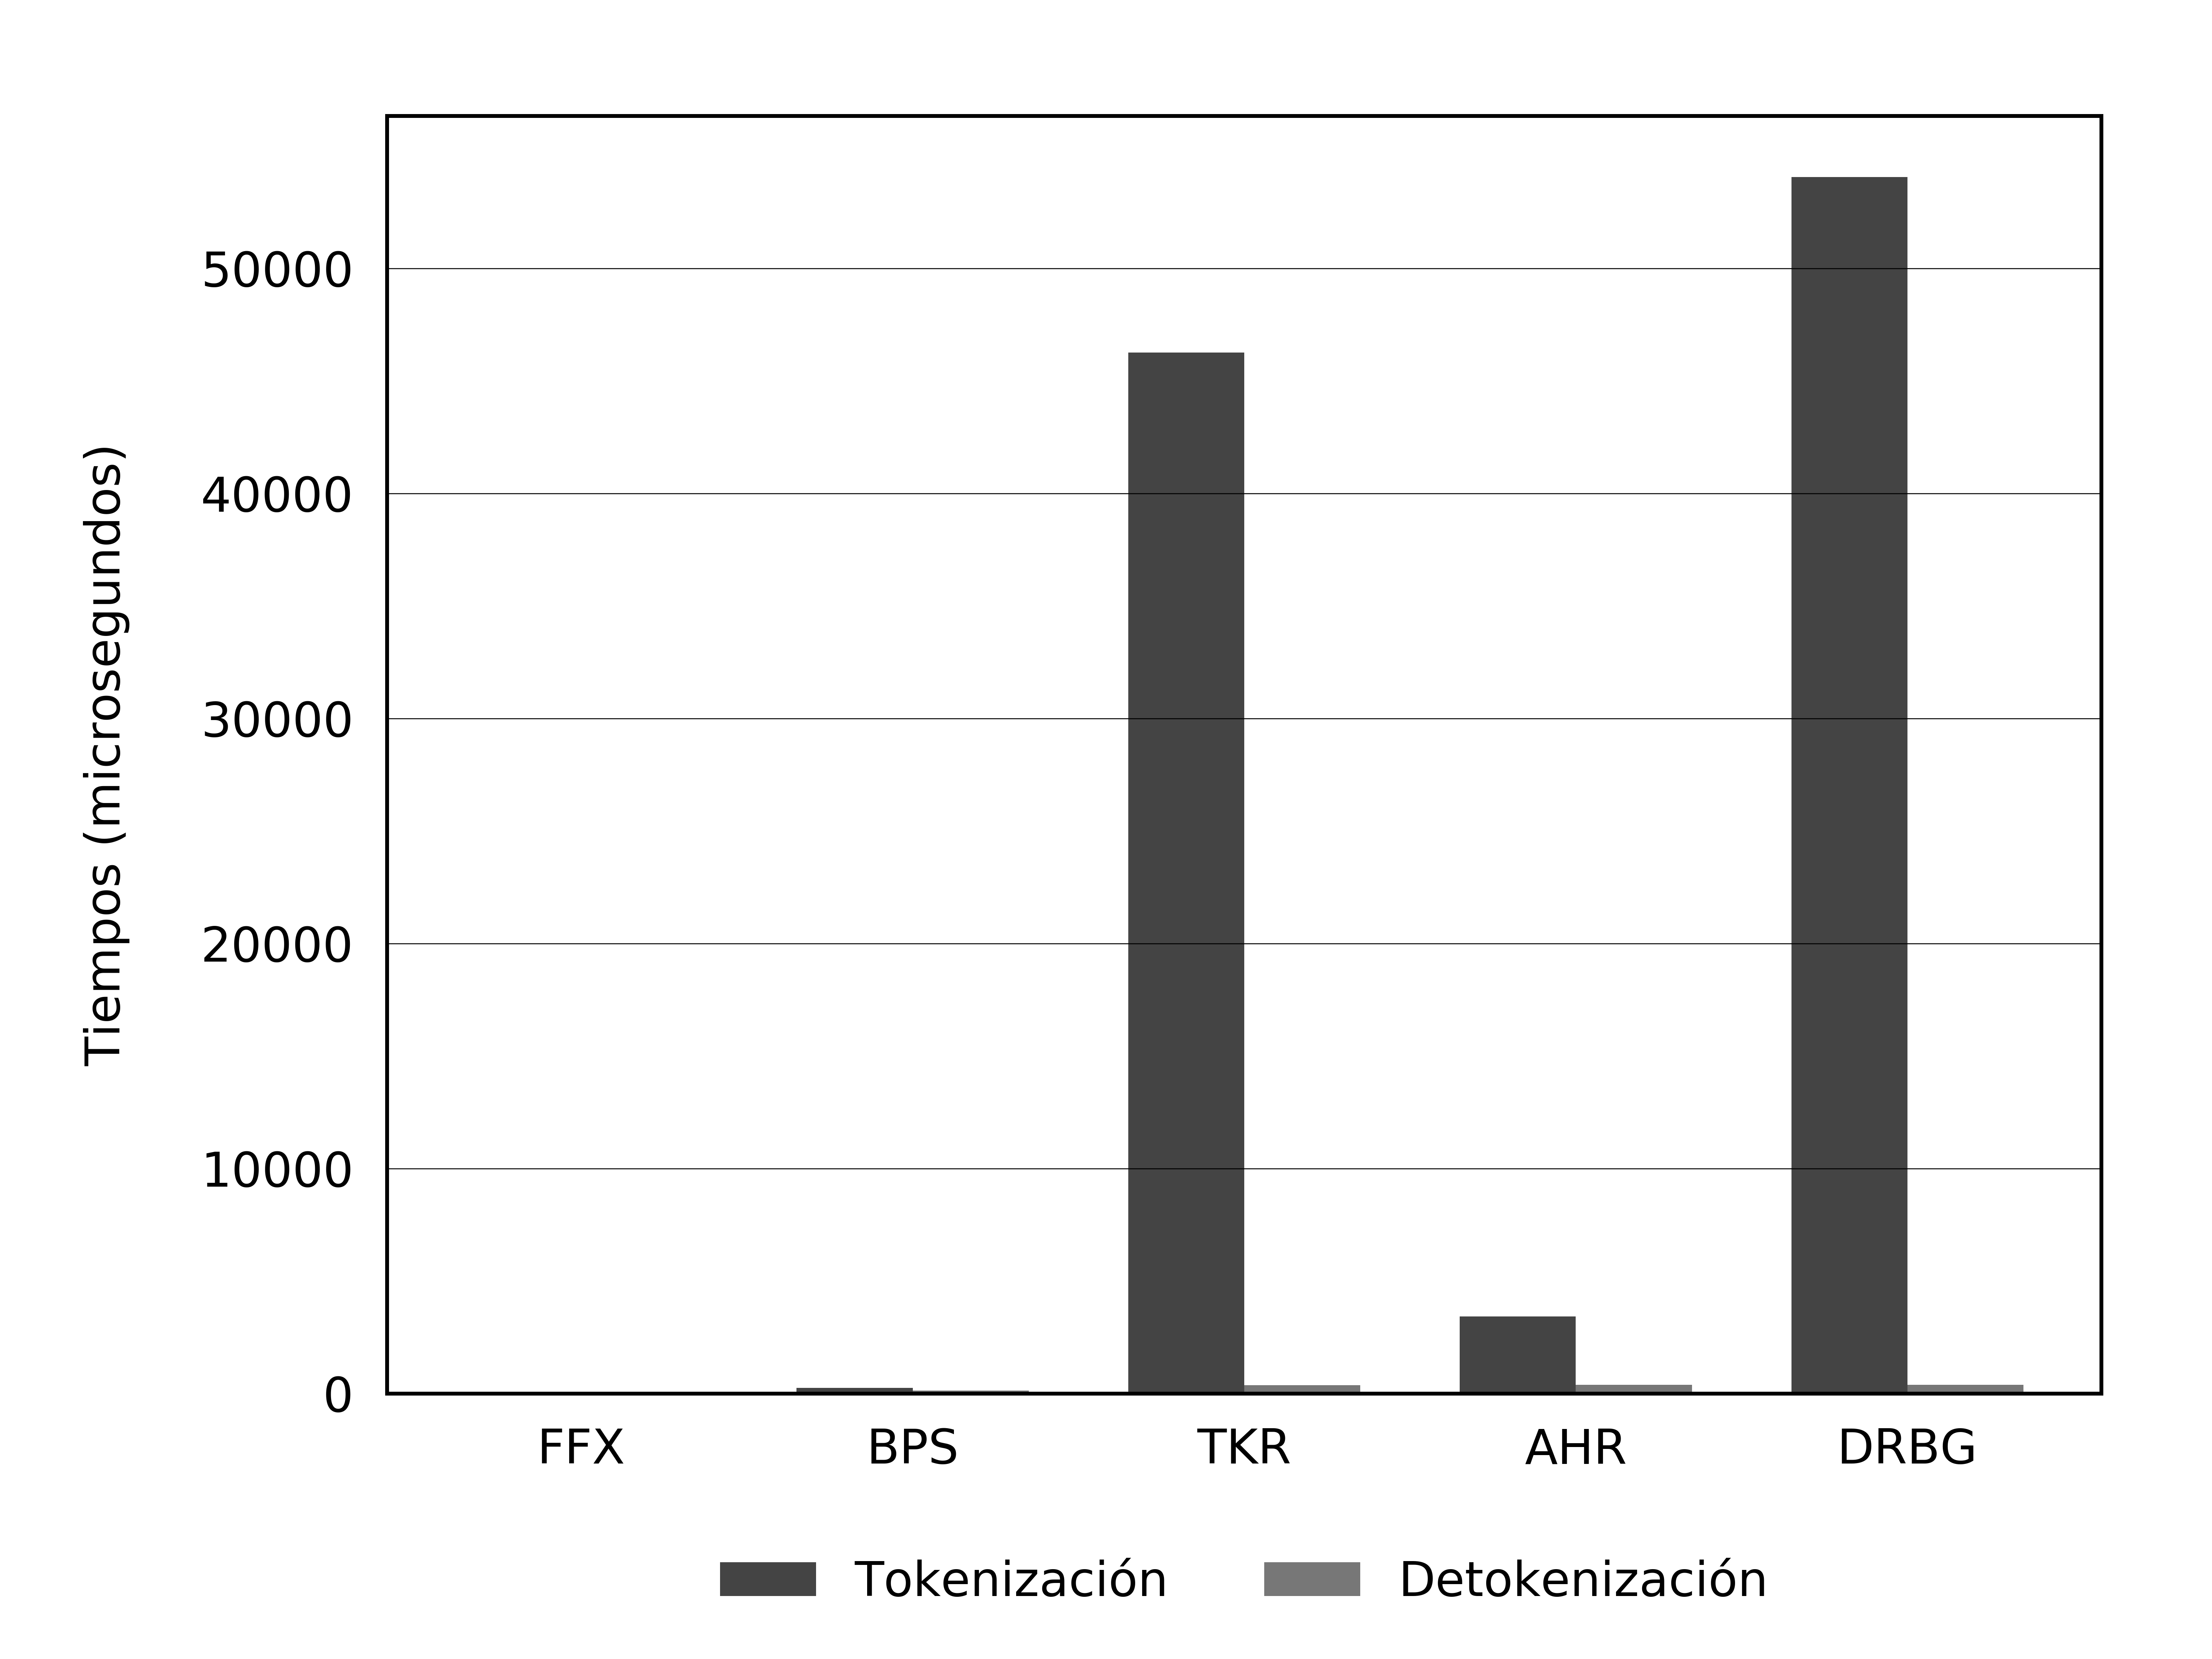
\includegraphics[width=0.5\linewidth]
        {articulo-rci/tiempos_unitarios.png}}
    \subfloat[Generación de tokens]{
      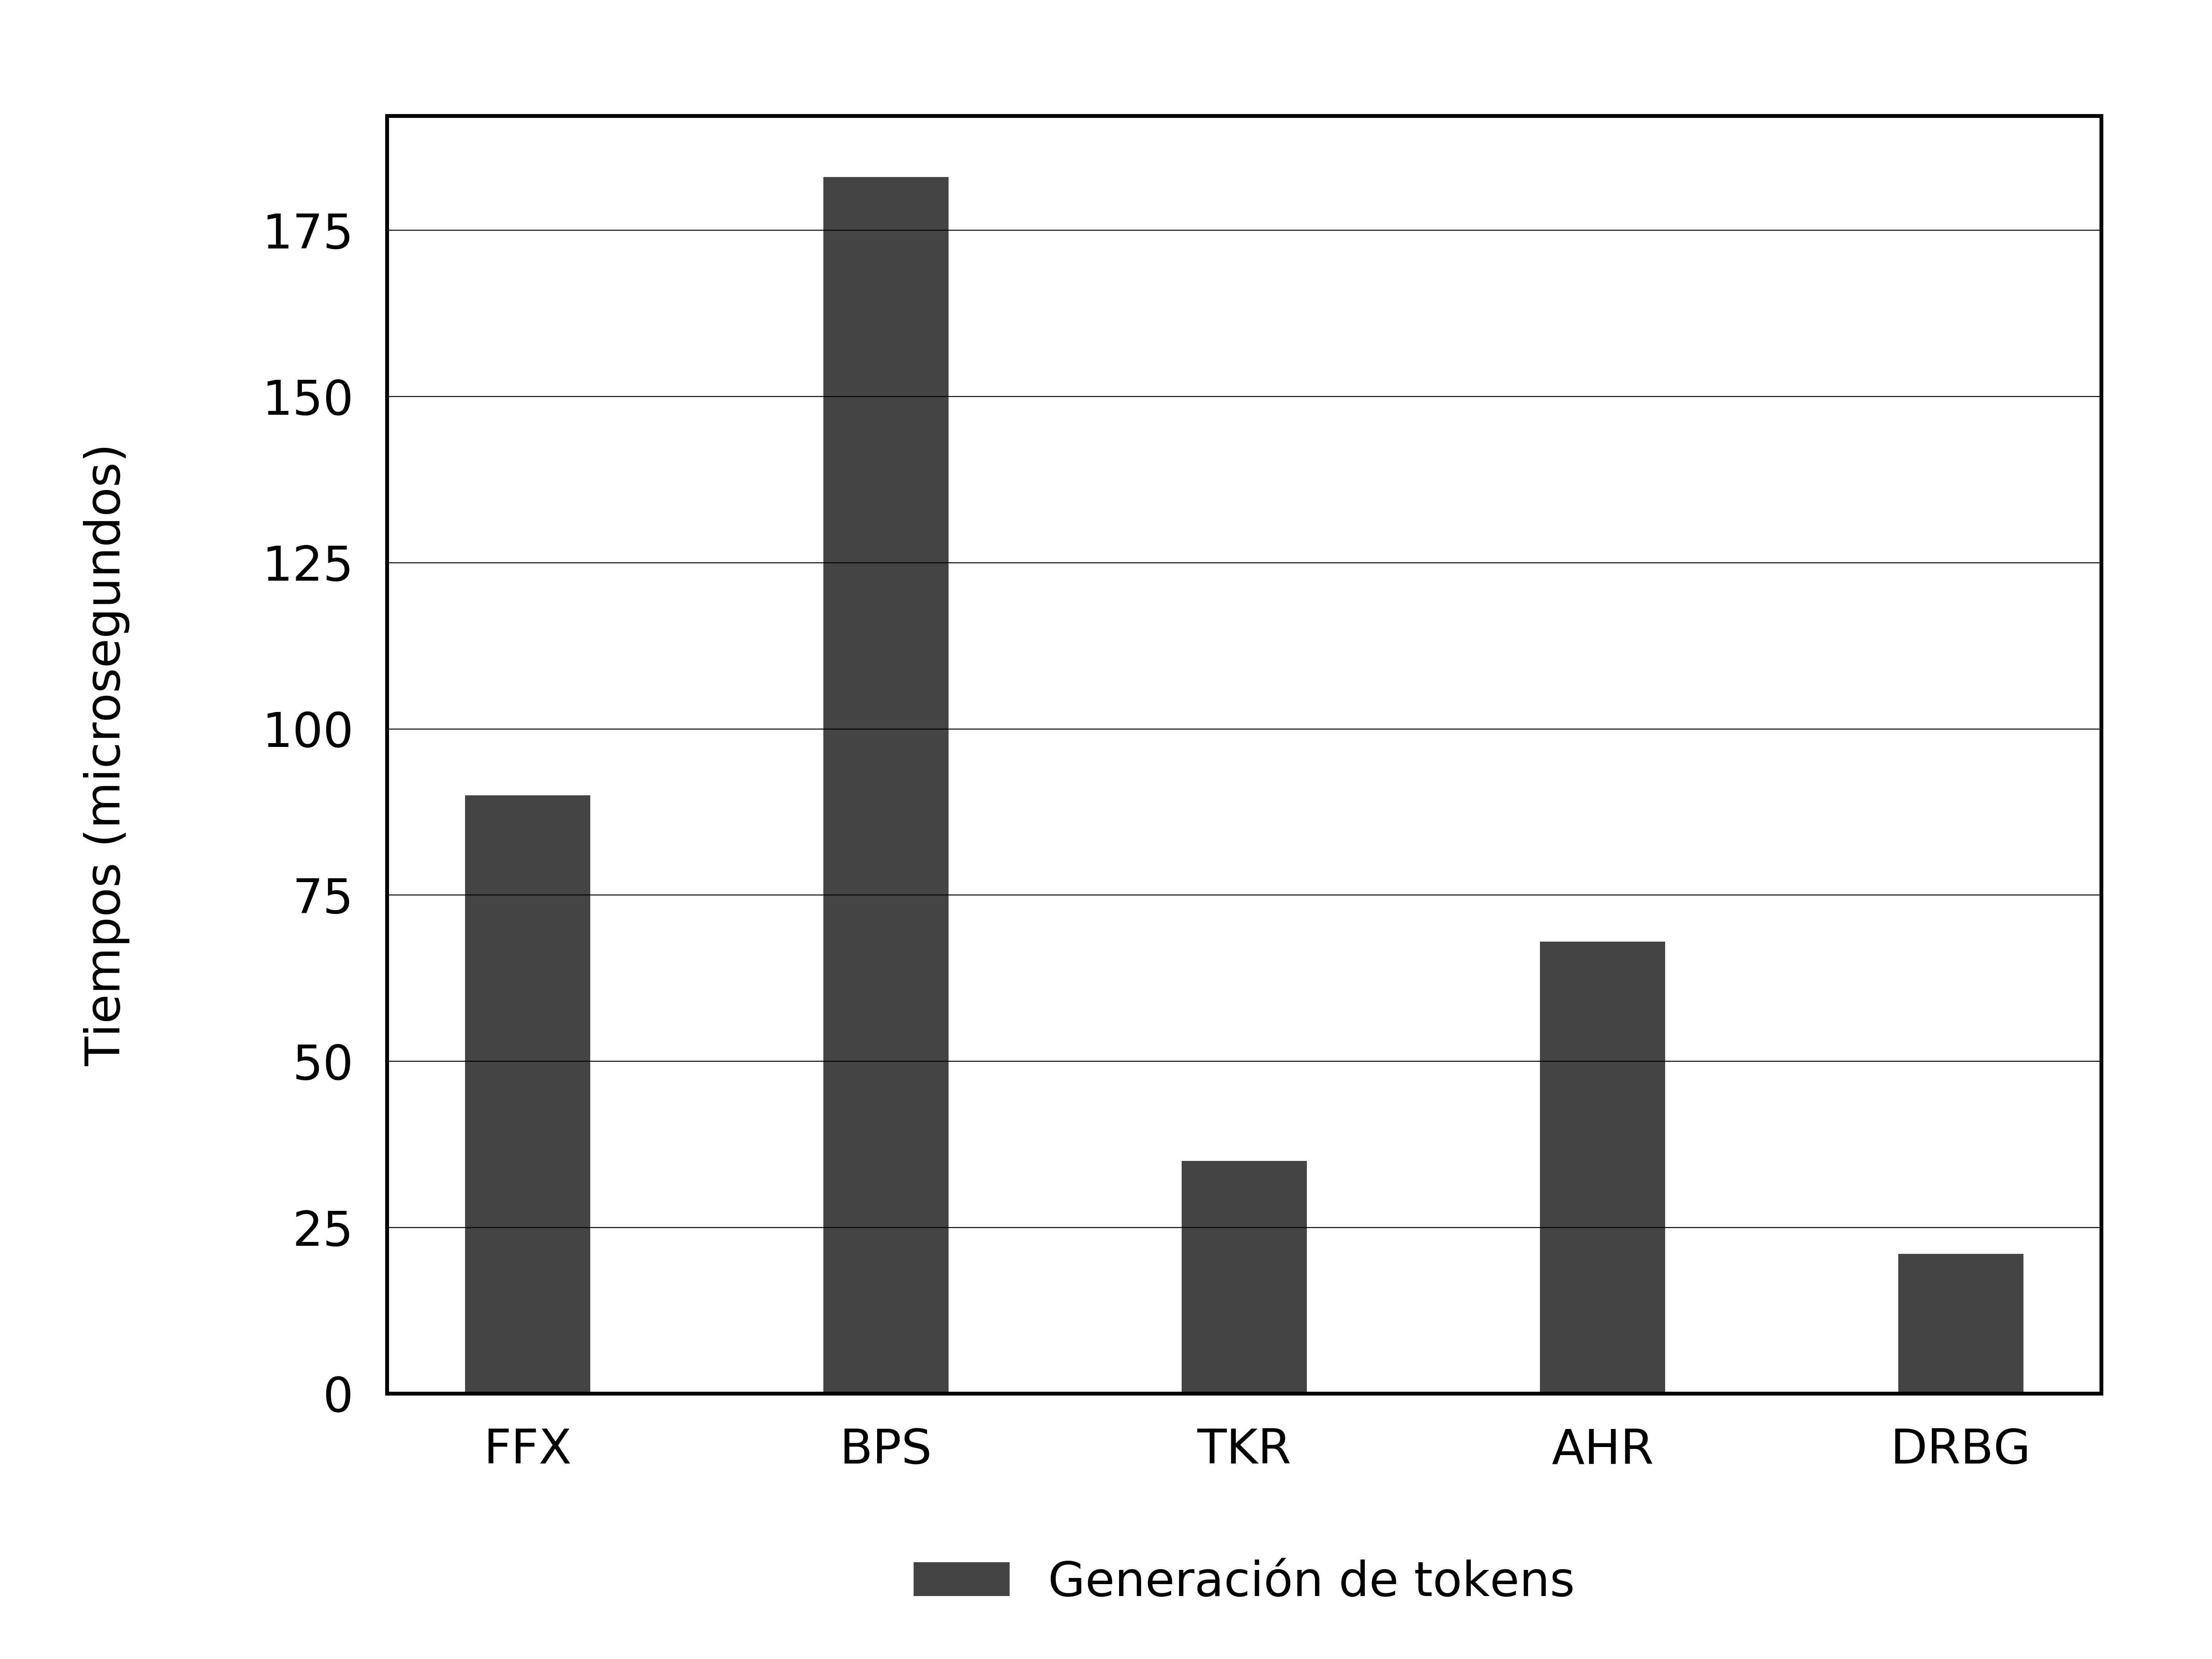
\includegraphics[width=0.5\linewidth]
        {articulo-rci/tiempos_tokenizacion.png}}
    \end{figure}
  \end{frame}

  \begin{frame}{Conclusiones}
    \begin{itemize}
      \item La tokenización es una aplicación de la criptografía.
      \item La denominación \textit{no criptográfica} del PCI es contradictoria.
    \end{itemize}
  \end{frame}

  \begin{frame}[allowframebreaks]{Bibliografía}
    \printbibliography
  \end{frame}

  % Espacio entre párrafos
  \setlength{\parskip}{0.0em}

  {\setbeamertemplate{footline}{}
  \frame{\titlepage}}

\end{document}
